\section{Results}\label{sec:results}

\subsection{Efficacy}

We demonstrate the efficacy of our autofocus algorithm by reproducing the
results in~\cite{ash2012autofocus}. We used the publicly released GOTCHA data
set from the Air Force Research Lab's Sensor Data Management System
~\cite{gotcha}. This data set contains multiple elevations of SAR data collected
in a circular aperture at 604 MHz bandwidth. For the following, we used
$25^{\circ}$ of azimuth with about 119 pulses per degree from the eighth pass.
As the available data set has been focused, we introduce phase errors in the
form of zero mean white Gaussian noise with a standard deviation of $\pi$
radians applied directly to each pulse in the phase history.
Fig.~\ref{fig:efficacy} depicts the results: The ideal image is shown
in~\subref{fig:ideal}, the noise-injected image in~\subref{fig:unfocused} and the
result of focusing in~\subref{fig:focused}.

\begin{figure}
  \centering
  \begin{subfigure}{0.5\textwidth}
    \centering
    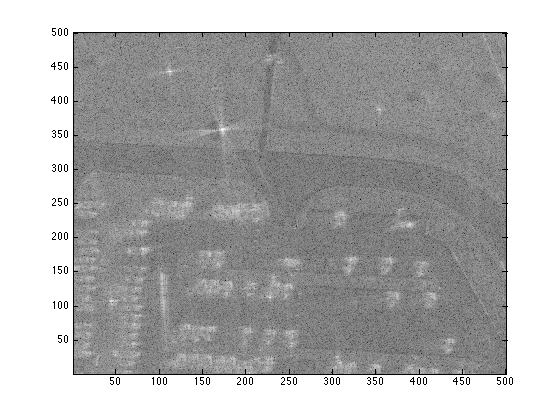
\includegraphics[width=\textwidth]{unfocused_noise_free_image.png}
    \caption{Unfocused image with no noise added.}
    \label{fig:ideal}
  \end{subfigure}
  \vfill
  \begin{subfigure}{0.5\textwidth}
    \centering
    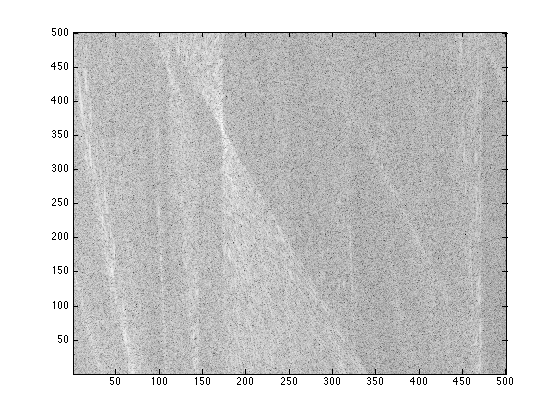
\includegraphics[width=\textwidth]{unfocused_noisy_image.png}
    \caption{Unfocused image with noise added.}
    \label{fig:unfocused}
  \end{subfigure}
  \vfill
  \begin{subfigure}{0.5\textwidth}
    \centering
    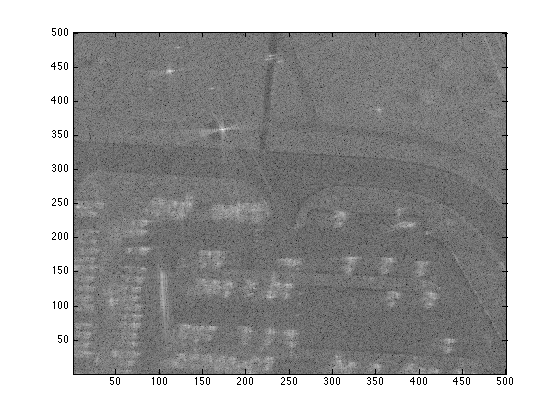
\includegraphics[width=\textwidth]{focused_image.png}
    \caption{Focused image.}
    \label{fig:focused}
  \end{subfigure}
  \vspace{5 mm}
  \caption{Gradient descent autofocus algorithm qualitative results}
  \label{fig:efficacy}
\end{figure}

\subsection{Performance}

This section explains our experimental methodology as well as presents and
discusses our findings. As discussed above, we used the GOTCHA dataset to
obtain performance measurements. In particular, we compared our implementations
against a parallel MATLAB reference implementation of gradient descent. We
measured performance as as function of pulse history size (degrees azimuth) as
well as added noise.

Our multithreaded experiments were conducted on 64 core, 2.5 GHz AMD Opteron
processors with 125 GB of RAM running Red Hat Enterprise Linux 6. For the GPU
experiments, we had access to a single Quadro K620 CUDA 5.0 card with 2 GB of
global memory, 1.12 GHz clock rate, and a memory bandwidth of 900 MHz. The host
possessed 4 Intel i5 cores at 3.3 GHz.

\subsubsection{Image Size}

The first experiment sought to characterize the performance scalability as a
function of input size. We measured the execution time as more degrees azimuth
were swept added to the phase history. Fig.~\ref{fig:speedup} depicts the
relative performance improvement for both the multithreaded CPU solution as well
as the GPU based solution. As shown, the GPU solution consistently surpasses the
CPU-only implementation until $9^{\circ}$ of azimuth or $1075$ pulses. Here, the
memory bandwidth limitations of the GPU throttle the performance benefits of the
massively parallel architecture. On average, the multithreaded and GPU
implementations achieved a speed up of nearly $32\times$ and $40\times$, respectively over
the parallelized MATLAB implementation, with as high as $53\times$ and $82\times$ for select
input sizes.

\begin{figure}
  \centering
  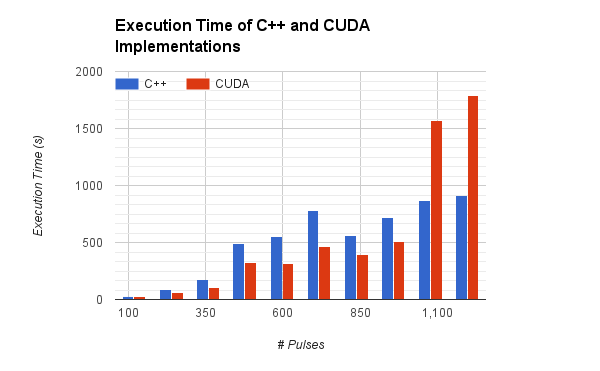
\includegraphics[width=0.5\textwidth]{speedup.png}
  \vspace{5 mm}
  \caption{Speed up of the C++ and CUDA implementations as a function of pulses.}
  \label{fig:speedup}
\end{figure}

\subsubsection{Noise Tolerance}

The second experiment aimed to explore the gradient descent's performance
tolerance as more noise was introduced into the phase history.
Fig.~\ref{fig:noise} depicts the normalized execution time of the
autofocus algorithms for $3^{\circ}$ of azimuth as the added noise varies
between $0$ and $3\pi$ radians. The data is normalized against zero added noise.
As can be seen from the graph, both implementations are relatively robust to
noise level, successfully minimizing entropy to a mean $9.344$ with standard
deviation of only $0.354$. The execution time similarly is stable, requiring an
average of $3.45$ and $4.08$ with standard deviations of $1.29$ and $1.74$ times
longer to converge for the C++ and CUDA implementations, respectively.

\begin{figure}
  \centering
  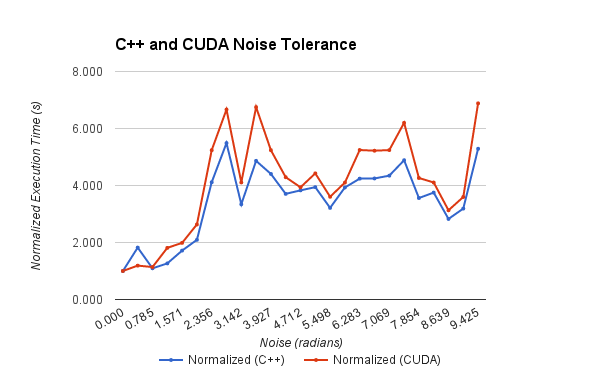
\includegraphics[width=0.5\textwidth]{noise.png}
  \vspace{5 mm}
  \caption{Execution time (s) of C++ and CUDA implementations as a function of
  noise.}
  \label{fig:noise}
\end{figure}
